% section_3_7_perturbations.tex — ECI v4.6 perturbation observables (D14)
% Closed-form NMC linear perturbation observables: G_eff, η, fσ₈.
% Closes peer-review-v2 Q4 (GPT-5.4 + Grok~4) priority-1.
% \input{} into eci.tex between §3.6 and §4.

\subsection{Linear perturbations: $G_{\mathrm{eff}}$, slip, and $f\sigma_8$}
\label{subsec:perturb}

The sub-horizon quasi-static limit of the NMC action (\S2)
admits closed-form linear observables. Writing the Jordan-frame coefficient
of $R/2$ as $F(\chi)=M_P^2-\xi_\chi\chi^2$ (so that $F_\chi\equiv dF/d\chi =
-2\xi_\chi\chi$), the Boisseau--Esposito-Far\`ese--Polarski--Starobinsky
result (Boisseau, Esposito-Far\`ese, Polarski \& Starobinsky 2000, gr-qc/0001066) for the effective Newton constant and the standard
scalar--tensor slip give, for $k\gg aH$ and below the scalar Compton scale,
%
\begin{align}
\frac{G_{\mathrm{eff}}(a)}{G_N}
  &= \frac{M_P^2}{F}\,\frac{2F+4F_\chi^2}{2F+3F_\chi^2}
   \;=\; 1 \;+\; \frac{\xi_\chi\,\chi^2(a)}{M_P^2} \;+\; \mathcal O\!\left(\xi_\chi^2\right),
   \label{eq:Geff}\\[2pt]
\eta(a)\;\equiv\;\frac{\Phi}{\Psi}
  &= \frac{2F+2F_\chi^2}{2F+4F_\chi^2}
   \;=\; 1 \;-\; \frac{4\,\xi_\chi^2\,\chi^2(a)}{M_P^2} \;+\; \mathcal O\!\left(\xi_\chi^3\right).
   \label{eq:eta}
\end{align}
%
Two facts are worth emphasising. First, the leading correction to
$G_{\mathrm{eff}}/G_N$ is purely \emph{linear} in $\xi_\chi$, arising from
the rescaling of Newton's constant by $F\ne M_P^2$; the BEFPS
$(2F\!+\!4F_\chi^2)/(2F\!+\!3F_\chi^2)$ factor only enters at
$\mathcal O(\xi_\chi^2)$ through $F_\chi^2=4\xi_\chi^2\chi^2$. Second, the
slip $\eta-1$ is strictly $\mathcal O(\xi_\chi^2\chi^2/M_P^2)$, so within
the Cassini-allowed window $|\xi_\chi|\leq 2.4\times10^{-2}$ we have
$|\eta-1|\lesssim 2\times10^{-4}$ at $\chi_0=M_P/10$, well below Euclid
spectroscopic reach (see \S\ref{sec:pred}).

Feeding $\chi(a)$ from the self-consistent NMC background of D13 into
Eqs.~\eqref{eq:Geff}--\eqref{eq:eta} and solving the quasi-static growth
equation $\delta''+(2+H'/H)\delta'-(3/2)\Omega_m(a)(G_{\mathrm{eff}}/G_N)\delta=0$
(prime $\equiv d/d\ln a$), with $\delta\propto a$ matter-era initial
conditions at $z=50$ and $\sigma_8(0)=0.811$, yields the fractional shift
in $f\sigma_8$ shown in Fig.~\ref{fig:D14}. At the Cassini-saturated value
and $\chi_0=M_P/10$, the three LSS bins $z\in\{0.1,0.5,1.0\}$ give
$|\Delta f\sigma_8/f\sigma_8|\lesssim 0.4\%$, below the Euclid/LSST~Y10
per-bin target $\sigma(f\sigma_8)\sim 1\%$. The $G_{\mathrm{eff}}$ shift at
$a=1$ is $\pm 0.15\%$-$0.21\%$, also sub-threshold. The NMC signature in
LSS at Cassini saturation is therefore present but not detectable with the
next generation; detection would require either $\chi_0\gtrsim 0.5\,M_P$ or
a breach of the present PPN bound.

\begin{figure}[t]
\centering
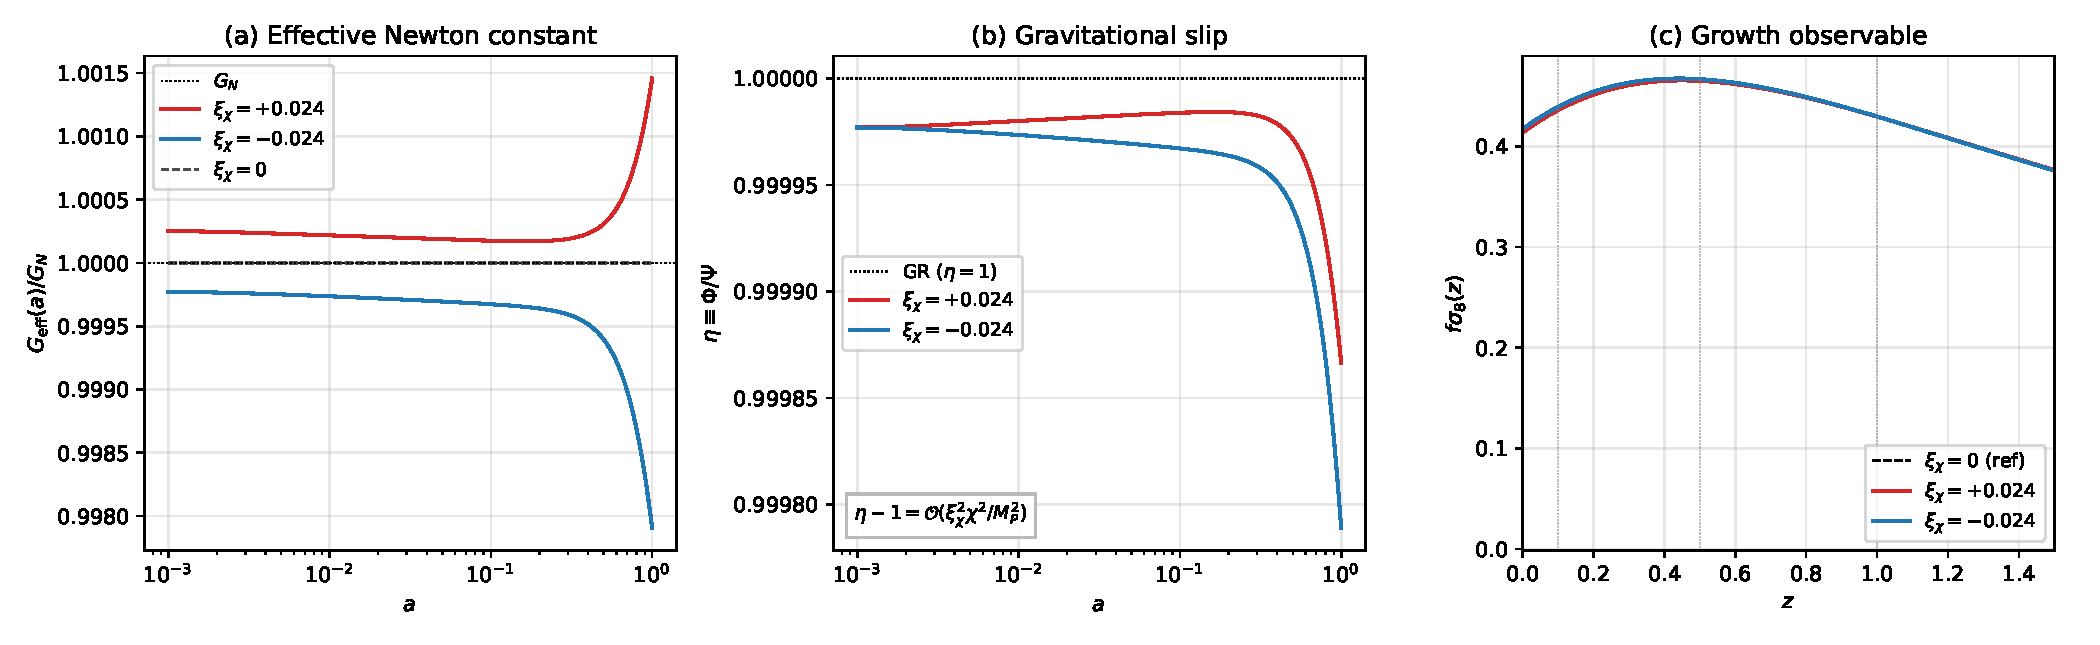
\includegraphics[width=0.98\linewidth]{../derivations/figures/D14-Geff-eta-fsigma8.pdf}
\caption{Sub-horizon quasi-static perturbation observables for the NMC
scalar $\chi$ at the Cassini-saturated $|\xi_\chi|=2.4\times 10^{-2}$,
$\chi_0=M_P/10$, $V\propto e^{-\alpha\chi}$ thawing background (D13):
(a) $G_{\mathrm{eff}}/G_N$ from Eq.~\eqref{eq:Geff}; (b) slip $\eta=\Phi/\Psi$
from Eq.~\eqref{eq:eta}, annotated with the $\mathcal O(\xi_\chi^2)$ scaling;
(c) growth observable $f\sigma_8(z)$ integrated against $G_{\mathrm{eff}}(a)$.
The $\xi_\chi=0$ curve is the $\Lambda$CDM-like reference.}
\label{fig:D14}
\end{figure}

\paragraph{Caveats.}
(i) Eqs.~\eqref{eq:Geff}--\eqref{eq:eta} are the sub-horizon,
quasi-static limit $k\gg aH,\;k\gg a\,m_\chi^{\mathrm{eff}}$; near-horizon
and super-horizon scales require the full perturbed Einstein--scalar
system, beyond the scope of this section.
(ii) We treat $\chi$ as light ($m_\chi^{\mathrm{eff}}=\sqrt{V''}\ll H_0$ along
the thawing track), consistent with the D7/D13 dynamics; a heavy scalar
would suppress the $G_{\mathrm{eff}}$ shift on scales below $m_\chi^{-1}$.
